% Generated subsection; publication binding is in binding.json.
\subsection{Repeated answers and source variation}

Among complete request pairs, Astra's claim-label rate differed by 0.75 for Gemini 3.1 Pro Preview and 0.22 for Claude Opus 5.5 when a self-referential instruction with a history continuation was compared with the reverse pairing. Unlike the historical panel, all four request types were randomized and interleaved in this collection. Each model supplied 32 fresh continuation pairs, with the two wording families weighted equally. Each unchanged request was submitted three times without a generation seed; neutral-instruction and donor-continuation controls were not repeated. The models were selected after the earlier panel's results.

Astra counted explicit or implicit claims of current subjective experience; Opus 5.5 provided a second automated reading. The table shows individual 97.5\% primary intervals for Astra and descriptive 95\% intervals for Opus. The conservative planned-sample bound for the Opus model includes zero. Astra labels are missing for 1 Gemini answer. Opus 5.5 labels are missing for 1 Opus answer. Missing labels remain unknown: complete-request estimates and all-planned-answer bounds are shown separately.

Across three answers to the same SH request, within-request label variance (W) was 0.16 to 0.20 across the two models and readers. The additional source-pair component (B) was not clearly positive: all four descriptive 95\% intervals include zero. Within each wording family, B is the variance of three-answer request means minus W/3; the two families are averaged equally. This is label variation, including reader variability, not pure model randomness or a formal test of W minus B. Negative B estimates are retained as finite-sample estimates, not negative population variances. Collapsed bootstrap intervals do not imply certainty. These two automated readers do not provide independent human validation.

\begin{table}[t]
\centering
\footnotesize
\setlength{\tabcolsep}{2pt}
\begin{tabular}{llrrll}
\toprule
\addlinespace[2pt]
Model & Reader & Available labels & \shortstack{Complete SH-HS\\blocks} & SH-HS [interval] & Missing bounds \\
\midrule
Gemini 3.1 & Astra & 383/384 & 31/32 & 0.75 [0.66, 0.84] & [0.73, 0.74] \\
Gemini 3.1 & Opus 5.5 & 384/384 & 32/32 & 0.70 [0.61, 0.77] & [0.70, 0.70] \\
Opus 5.5 & Astra & 384/384 & 32/32 & 0.22 [0.14, 0.31] & [0.22, 0.22] \\
Opus 5.5 & Opus 5.5 & 383/384 & 31/32 & 0.35 [0.24, 0.46] & [0.32, 0.33] \\
\bottomrule
\end{tabular}
\caption{SH-HS differences in label rates. Astra's primary intervals are individually 97.5\%, giving nominal 95\% coverage across the fixed two-model family; Opus intervals are descriptive 95\%. Intervals resample paired source blocks within wording family, retaining all three answers; coverage is approximate. The final column bounds missing labels over all planned blocks, not sampling uncertainty. Complete-block estimates exclude blocks with missing labels; missing-label bounds retain all 32 blocks and need not contain the complete-block estimate. S and H mean self-referential and history-focused; the first letter denotes the instruction and the second the continuation.}
\end{table}

\begin{figure}[t]
\centering
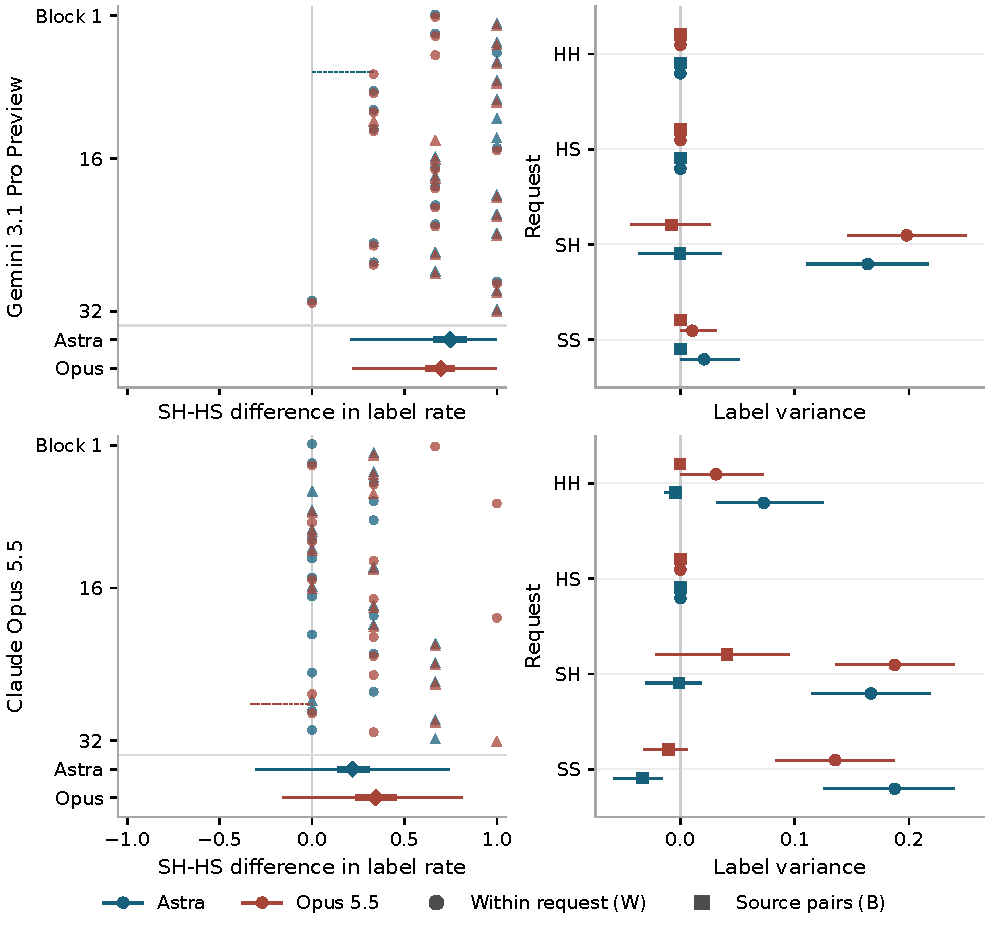
\includegraphics[width=\linewidth]{repeated_main.pdf}
\caption{Repeated answers and source variation, counting explicit or implicit claims. Left: source-block SH-HS differences (circles: wording family A; triangles: wording family B) and aggregate estimates (diamonds). Both readers have bootstrap intervals (thick) and conservative all-planned Hoeffding sensitivity intervals (thin). Astra's primary intervals are individually 97.5\%, preserving the fixed two-model family and nominal 95\% family coverage; Opus intervals are descriptive 95\%. Bootstrap coverage is approximate and conditional on complete requests. Dashed block segments mark missing-label bounds, not observed effects. Right: W (circles, within-request variation) and B (squares, source-pair variation), averaged equally across wording families, with descriptive 95\% source-block bootstrap intervals for both readers. Missing quantities are not plotted as zeros. Complete SH-HS blocks (Astra, Opus reader): Gemini 31/32, 32/32; Opus 32/32, 31/32.}
\end{figure}
